\documentclass{beamer}
\usepackage[utf8]{inputenc}
\usepackage{setspace}
\usepackage{hyperref}
\usepackage{amsmath}
\usepackage{pifont}
\usepackage{color}
% Just add % Just add % Just add \input{smalltalkEnv} to your file
% then you can use :
% \begin{lstlisting}[language=Smalltalk]
% false become: true.
% \end{lstlisting}

\usepackage{color}
\usepackage{listings}
\usepackage{etoolbox}
\usepackage{textcomp}

\definecolor{stComment}{rgb}{0.5,0.5,0.5}
\definecolor{stString}{rgb}{0.58,0,0.82}
\definecolor{stKeywords}{rgb}{0.21,0.55,0.7}
\definecolor{stNumbers}{rgb}{.5,0,0}

\newtoggle{InString}{}% Keep track of if we are within a string
\togglefalse{InString}% Assume not initally in string
\newcommand*{\ColorIfNotInString}[1]{\iftoggle{InString}{#1}{\color{stNumbers}#1}}%
\newcommand*{\ProcessQuote}[1]{#1\iftoggle{InString}{\global\togglefalse{InString}}{\global\toggletrue{InString}}}%

\lstdefinelanguage{Smalltalk}{
  keywordstyle=\color{stKeywords},
  commentstyle=\color{stComment},
  stringstyle=\color{stString},
  alsoletter=\#,
  identifierstyle=\idstyle, 
  showstringspaces=false,
  morekeywords={true,false,self,super,nil},
  sensitive=true, 
  morecomment=[s]{"}{"}, 
  morestring=[d]', 
  style=SmalltalkStyle,
  tabsize=2,
  basicstyle=\ttfamily,
  upquote=true,
}


\makeatletter%
\newcommand*\idstyle[1]{%
  \expandafter\id@style\the\lst@token{#1}\relax%
}
\def\id@style#1#2\relax{%
  \ifnum\pdfstrcmp{#1}{\#}=0%
  \ttfamily\color{stString} \the\lst@token%
  \else%
  \edef\tempa{\uccode`#1}%
  \edef\tempb{`#1}%
  \ifnum\tempa=\tempb%
  \ttfamily\color{blue} \the\lst@token%
  \else%
  \the\lst@token%
  \fi%
  \fi%
}

\lstdefinestyle{SmalltalkStyle}{ 
  literate=%
  {^}{{$\uparrow$}}1% 
  % {"}{{{\ProcessQuote{"}}}}1% Disable coloring within double quotes
  % {'}{{{\ProcessQuote{'}}}}1% Disable coloring within single quote
  {0}{{{\ColorIfNotInString{0}}}}1%
  {1}{{{\ColorIfNotInString{1}}}}1%
  {2}{{{\ColorIfNotInString{2}}}}1%
  {3}{{{\ColorIfNotInString{3}}}}1%
  {4}{{{\ColorIfNotInString{4}}}}1%
  {5}{{{\ColorIfNotInString{5}}}}1%
  {6}{{{\ColorIfNotInString{6}}}}1%
  {7}{{{\ColorIfNotInString{7}}}}1%
  {8}{{{\ColorIfNotInString{8}}}}1%
  {9}{{{\ColorIfNotInString{9}}}}1%
} 
 to your file
% then you can use :
% \begin{lstlisting}[language=Smalltalk]
% false become: true.
% \end{lstlisting}

\usepackage{color}
\usepackage{listings}
\usepackage{etoolbox}
\usepackage{textcomp}

\definecolor{stComment}{rgb}{0.5,0.5,0.5}
\definecolor{stString}{rgb}{0.58,0,0.82}
\definecolor{stKeywords}{rgb}{0.21,0.55,0.7}
\definecolor{stNumbers}{rgb}{.5,0,0}

\newtoggle{InString}{}% Keep track of if we are within a string
\togglefalse{InString}% Assume not initally in string
\newcommand*{\ColorIfNotInString}[1]{\iftoggle{InString}{#1}{\color{stNumbers}#1}}%
\newcommand*{\ProcessQuote}[1]{#1\iftoggle{InString}{\global\togglefalse{InString}}{\global\toggletrue{InString}}}%

\lstdefinelanguage{Smalltalk}{
  keywordstyle=\color{stKeywords},
  commentstyle=\color{stComment},
  stringstyle=\color{stString},
  alsoletter=\#,
  identifierstyle=\idstyle, 
  showstringspaces=false,
  morekeywords={true,false,self,super,nil},
  sensitive=true, 
  morecomment=[s]{"}{"}, 
  morestring=[d]', 
  style=SmalltalkStyle,
  tabsize=2,
  basicstyle=\ttfamily,
  upquote=true,
}


\makeatletter%
\newcommand*\idstyle[1]{%
  \expandafter\id@style\the\lst@token{#1}\relax%
}
\def\id@style#1#2\relax{%
  \ifnum\pdfstrcmp{#1}{\#}=0%
  \ttfamily\color{stString} \the\lst@token%
  \else%
  \edef\tempa{\uccode`#1}%
  \edef\tempb{`#1}%
  \ifnum\tempa=\tempb%
  \ttfamily\color{blue} \the\lst@token%
  \else%
  \the\lst@token%
  \fi%
  \fi%
}

\lstdefinestyle{SmalltalkStyle}{ 
  literate=%
  {^}{{$\uparrow$}}1% 
  % {"}{{{\ProcessQuote{"}}}}1% Disable coloring within double quotes
  % {'}{{{\ProcessQuote{'}}}}1% Disable coloring within single quote
  {0}{{{\ColorIfNotInString{0}}}}1%
  {1}{{{\ColorIfNotInString{1}}}}1%
  {2}{{{\ColorIfNotInString{2}}}}1%
  {3}{{{\ColorIfNotInString{3}}}}1%
  {4}{{{\ColorIfNotInString{4}}}}1%
  {5}{{{\ColorIfNotInString{5}}}}1%
  {6}{{{\ColorIfNotInString{6}}}}1%
  {7}{{{\ColorIfNotInString{7}}}}1%
  {8}{{{\ColorIfNotInString{8}}}}1%
  {9}{{{\ColorIfNotInString{9}}}}1%
} 
 to your file
% then you can use :
% \begin{lstlisting}[language=Smalltalk]
% false become: true.
% \end{lstlisting}

\usepackage{color}
\usepackage{listings}
\usepackage{etoolbox}
\usepackage{textcomp}

\definecolor{stComment}{rgb}{0.5,0.5,0.5}
\definecolor{stString}{rgb}{0.58,0,0.82}
\definecolor{stKeywords}{rgb}{0.21,0.55,0.7}
\definecolor{stNumbers}{rgb}{.5,0,0}

\newtoggle{InString}{}% Keep track of if we are within a string
\togglefalse{InString}% Assume not initally in string
\newcommand*{\ColorIfNotInString}[1]{\iftoggle{InString}{#1}{\color{stNumbers}#1}}%
\newcommand*{\ProcessQuote}[1]{#1\iftoggle{InString}{\global\togglefalse{InString}}{\global\toggletrue{InString}}}%

\lstdefinelanguage{Smalltalk}{
  keywordstyle=\color{stKeywords},
  commentstyle=\color{stComment},
  stringstyle=\color{stString},
  alsoletter=\#,
  identifierstyle=\idstyle, 
  showstringspaces=false,
  morekeywords={true,false,self,super,nil},
  sensitive=true, 
  morecomment=[s]{"}{"}, 
  morestring=[d]', 
  style=SmalltalkStyle,
  tabsize=2,
  basicstyle=\ttfamily,
  upquote=true,
}


\makeatletter%
\newcommand*\idstyle[1]{%
  \expandafter\id@style\the\lst@token{#1}\relax%
}
\def\id@style#1#2\relax{%
  \ifnum\pdfstrcmp{#1}{\#}=0%
  \ttfamily\color{stString} \the\lst@token%
  \else%
  \edef\tempa{\uccode`#1}%
  \edef\tempb{`#1}%
  \ifnum\tempa=\tempb%
  \ttfamily\color{blue} \the\lst@token%
  \else%
  \the\lst@token%
  \fi%
  \fi%
}

\lstdefinestyle{SmalltalkStyle}{ 
  literate=%
  {^}{{$\uparrow$}}1% 
  % {"}{{{\ProcessQuote{"}}}}1% Disable coloring within double quotes
  % {'}{{{\ProcessQuote{'}}}}1% Disable coloring within single quote
  {0}{{{\ColorIfNotInString{0}}}}1%
  {1}{{{\ColorIfNotInString{1}}}}1%
  {2}{{{\ColorIfNotInString{2}}}}1%
  {3}{{{\ColorIfNotInString{3}}}}1%
  {4}{{{\ColorIfNotInString{4}}}}1%
  {5}{{{\ColorIfNotInString{5}}}}1%
  {6}{{{\ColorIfNotInString{6}}}}1%
  {7}{{{\ColorIfNotInString{7}}}}1%
  {8}{{{\ColorIfNotInString{8}}}}1%
  {9}{{{\ColorIfNotInString{9}}}}1%
} 

\usetheme{AnnArbor}


% My preferences
\graphicspath{{images/}}
\newcommand{\tip}{\boldmath{\textcolor{red}{$\Rightarrow$}}}
\newcommand{\drgeo}{Dr.~Geo}
\newcommand{\cmark}{\text{\ding{51}}}
\newcommand{\xmark}{\text{\ding{55}}}

\title{GUI application\\ with\\ Cuis-Smalltalk}

\author{Hilaire Fernandes}
\institute[DIP, Geneva]{Department of Public Instruction \\ Geneva}
\titlegraphic{
  
\includegraphics[width=2cm]{ArmoirieGeneve.png}
}
\date{November 2023}

\begin{document}
\begin{frame}
  \titlepage
\end{frame}
%
\begin{frame}{About me}
  \fontsize{12pt}{30pt}\selectfont
  \begin{itemize}
  \item Educator in public school, Geneva, B.Math, Ma.Ed
  \item Computer scientist, Ma.CS, PhD.CS
  \item Free software enthusiast and user since 1998
  \item And of course, Smalltalk user since 2002
  \end{itemize}
\end{frame}
%
\begin{frame}{Contents}
  \tableofcontents[hideallsubsections]
\end{frame}

\section{Why this workshop?}
\subsection{The intents}
\begin{frame}{Why writing a GUI application with \textbf{Smalltalk}?}

  \begin{itemize}
  \item Portable application
  \item Rapid prototyping
  \item To explore concepts and new ideas
  \item To learn from the environment itself
  \item Culture of design patterns
  \item Culture of testing
  \item Moldable environment
  \item Bugs hunt is fun, and fixes too
  \end{itemize}
\end{frame}
%
\begin{frame}{Why writing a GUI application with \textbf{Cuis}-Smalltalk?}

  \begin{itemize}
  \item A libre Smalltalk, it ensures \alert{the four fundamental freedoms}:
    \begin{enumerate}
    \item to run it,
    \item to study and to modify it,
    \item to distribute copy of it,
    \item to distribute modified version of it.
    \end{enumerate}
     
  \item A Smalltalk system for humble human being\\
    \tip\ system complexity under control, not on your way
  \item Cuis's \alert{Morph mark III} makes Morph correct \\
    \tip\ hierarchy, coordinates system, floating point precision
  \item State of the art \alert{Vector Graphics} engine \\
    \tip\ make your app beautifully 
  \item Develop your own vector widget \\
    \tip\ with \textsc{SVG} icons
  \end{itemize}
\end{frame}
%
\begin{frame}{A guide for the beginners}
  These workshop and related documents:
  \begin{itemize}
  \item A step by step guide to get started elaborating a Cuis App
  \item How to organize your code
  \item Expose the different parts needed for a Cuis App,
  \item Which packages to rely on
  \item Which design patterns you may want to use
  \item \emph{How to write your own vector widget} \tip\ sorry not this time
  \item Which resources to use
  \end{itemize}
\end{frame}

\subsection{The learning example}
\begin{frame}{An image viewer}
  Application with toolbar to view image and to operate
  transformations with undo/redo commands (World Menu-New Morph, AppView).
\begin{center}
  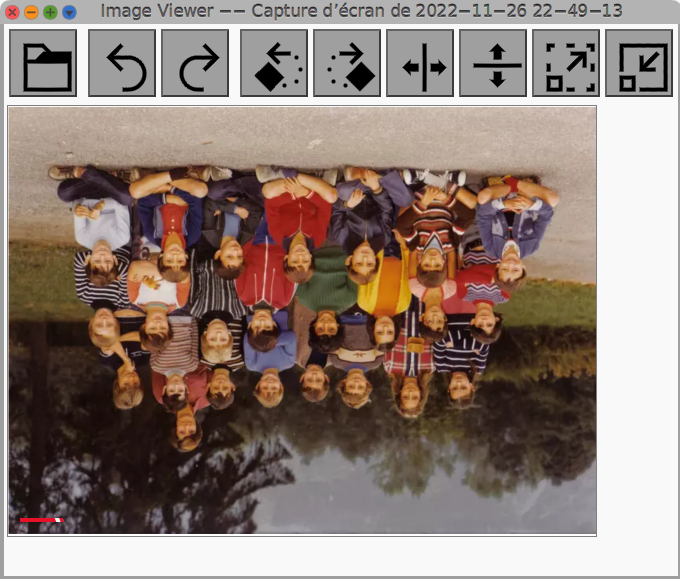
\includegraphics[width=0.6\textwidth]{CuisApp.png}
\end{center}
\end{frame}
%
\begin{frame}{How to follow the workshop?}
  Don't take note or use your computer, only write down this url for later use.
  \vspace*{2cm}
  \fontsize{16pt}{8pt}\selectfont
  \begin{center}
   \url{https://github.com/hilaire/CuisApp}
  \end{center}
  \fontsize{11pt}{8pt}\selectfont
  \vspace*{2cm}
  \begin{flushright}
   Enjoy the ride!
 \end{flushright}
\end{frame}

\section{Organise your disk}
\begin{frame}[fragile]{From scratch}
  The free operating system GNU/Linux is used along some Bash commands
  and scripts. You also need the \texttt{git} tool to access the Cuis
  repositories. Mac OS X should be fine.

  On Windows, you need to adapt the Bash script to Microsfoft shell.

\vspace{10pt}
  
  \tip\ In your disk, create a new folder ``\texttt{myProject}'' for
  your project:
\begin{verbatim}
    mkdir myProject
\end{verbatim}

  This is the place where you will pull the needed Cuis repositories,
  the virtual machine and the repository dedicated to your Cuis App.
\end{frame}

\subsection{Repositories \& VM}
% which basic repositories
\begin{frame}[fragile]{Cuis image}
  We need to clone the Cuis official repo to get the latest image and
  updates along additional repositories of libraries we want to
  use. We suggest you read latter the official guides to keep this
  repository updated\cite{cuisRepo}.

%\fontsize{10pt}{8pt}\selectfont
\begin{verbatim}
cd myProject
git clone --depth 1 \
   https://github.com/Cuis-Smalltalk/Cuis-Smalltalk-Dev.git
cd Cuis-Smalltalk-Dev
./clonePackageRepos.sh
\end{verbatim}
\end{frame}
%
\begin{frame}[fragile]{Virtual Machine}
  Get the latest virtual machine for GNU/Linux\cite{cuisRepo}:
\begin{verbatim}
cd myProject
rm -r cogspur
wget -O cogspur.tgz \
   https://github.com/OpenSmalltalk/opensmalltalk-vm/\
   releases/latest/download/squeak.cog.spur_linux64x64.tar.gz
tar -zxvf cogspur.tgz
mv ./sqcogspur64linuxht ./cogspur
\end{verbatim}
  
\tip\ Test you can start Cuis:
\begin{verbatim}
../cogspur/squeak Cuis6.0-6xxx
\end{verbatim}
\end{frame}
%
\begin{frame}[fragile]{Additional repositories}
  We want to install the SVG \& Cuis-Smalltalk-UI repositories:
%\fontsize{10pt}{8pt}\selectfont
\begin{verbatim}
cd myProject
git clone --depth 1 https://github.com/Cuis-Smalltalk/\
   Cuis-Smalltalk-UI.git
git clone --depth 1 https://github.com/Cuis-Smalltalk/\
   SVG.git
git clone --depth 1 https://github.com/Cuis-Smalltalk/\
   Numerics.git
\end{verbatim}

  It installs the repositories \texttt{Cuis-Smalltalk-UI} and
  \texttt{SVG} as folders in \texttt{myProject/}. They contains
  package files \texttt{.pck.st}.
  
\end{frame}
%
\begin{frame}[fragile]{CuisApp}
  Cuis is repository agnostic. Use whatever suits you to manage your
  Cuis app code\footnote[frame]{ For \drgeo\ I use Bazaar/Launchpad
    because it offers a web tool to edit translations in native
    languages\cite{drgeoRepo}}.

  \tip\ For your \alert{myApp}, you just clone its repository in the
  Cuis-Smalltalk-Dev folder:

\begin{verbatim}
cd myProject/Cuis-Smalltalk-Dev
git clone http://github.com/hilaire/CuisApp
\end{verbatim}

  \tip\ All the source codes and related resources needed for our Cuis
  application will go there.
  
\end{frame}

\subsection{App space}
% your dev App folder/repo
%
\begin{frame}[fragile]{Folders}

  We need places for the source code, scripts, resources,
  i18n(Internationalization), build:
\begin{verbatim}
cd myProject/Cuis-Smalltalk-Dev/CuisApp
mkdir src i18n build
mkdir -p resources/graphics/icons resources/doc
\end{verbatim}  
\end{frame}
%
\section{Packages}
% App template, GUI, SVG, locale, gettext
\subsection{Cuis packaging}
\begin{frame}[fragile]
  In a Cuis workspace, you request a package as a Feature:
  \begin{lstlisting}[language=Smalltalk]
    Feature require: 'UI-Components'
  \end{lstlisting}
  This installs the UI-Components package and more. It comes from the
  \texttt{Cuis-Smalltalk-UI/lib} repository.

  \vspace*{10pt}
  In fact it is a meta-package, read it:
  \fontsize{10pt}{8pt}\selectfont
  \begin{lstlisting}[language=Smalltalk]
    !provides: 'UI-Components' 1 4!
    !requires: 'Cuis-Base' 60 5032 nil!
    !requires: 'UI-DragAndDrop' 1 0 nil!
    !requires: 'UI-Entry' 1 3 nil!
    !requires: 'UI-Click-Select' 1 1 nil!
    !requires: 'UI-Panel' 1 5 nil!
    !requires: 'UI-Widgets' 1 0 nil!
  \end{lstlisting}
\end{frame}
\subsection{Package manager}
\begin{frame}
  Open it from the menu in the world World-Open-Installed Packages:
  \begin{center}
    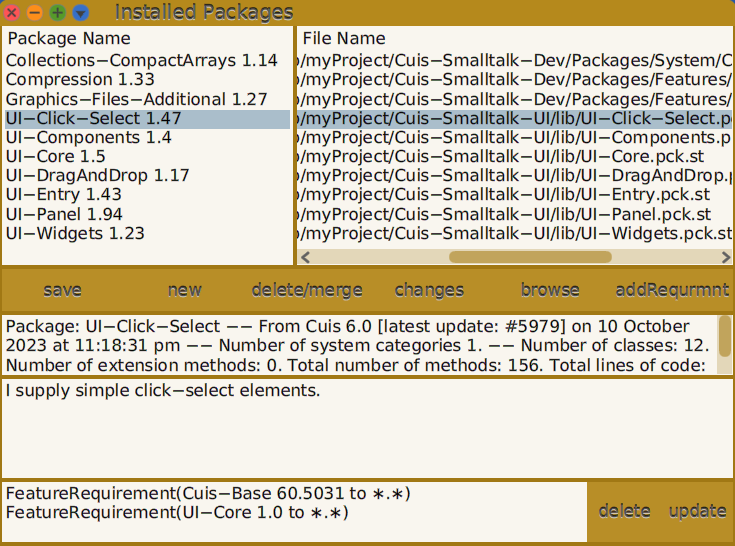
\includegraphics[width=0.8\textwidth]{PackageManager.png}    
  \end{center}
\end{frame}
%
\begin{frame}[fragile]{Our CuisApp package}
  To manage the code of our CuisApp, we create a package ``CuisApp''
  and add the dependent packages we need:
\fontsize{10pt}{8pt}\selectfont

\begin{lstlisting}[language=Smalltalk]
| package |
package := CodePackage
   named: 'CuisApp'
   createIfAbsent: true
   registerIfNew: true.
package featureSpec 
   requires: (FeatureRequirement name: 'SVG');
   requires: (FeatureRequirement name: 'UI-Components');
   requires: (FeatureRequirement name: 'Goodies');
   requires: (FeatureRequirement name: 'Gettext').
package save
  \end{lstlisting}

  \tip\ The package is saved along the Cuis image, in
  Cuis-Smalltalk-Dev.
\end{frame}

\begin{frame}{Package content}
  In the class browser, we create a CuisApp class in the category \textbf{CuisApp}.\\
  \tip\ All classes in the categories \texttt{CuisApp} and
  \texttt{CuisApp-\#\#\#} are automatically part of the CuisApp
  package. All the methods in the system categorized as
  \texttt{*CuisApp} are also part of the CuisApp package.
  \vspace*{10pt}

  Observe in the package manager the dependencies and the * indicating
  there are changes in the CuisApp package:
  \begin{center}
    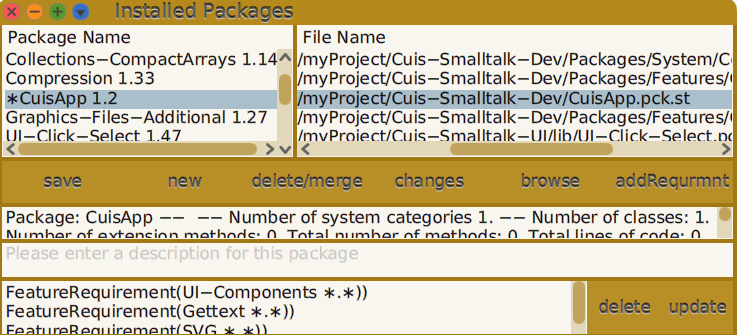
\includegraphics[width=0.7\textwidth]{CuisAppPackage.png}
  \end{center}
\end{frame}

\section{IDE}
% Customize, automate its setup
\subsection{Preparation}
\begin{frame}[fragile]
  Test our package:
    \begin{itemize}
    \item From the package manager, save once more the CuisApp
      package, then move its file \texttt{CuisApp.pck.st} in
      \texttt{CuisApp/src}, in the CuisApp repository.
    \item Quit Cuis without saving
    \item Restart Cuis and in a workspace execute:
\begin{lstlisting}[language=Smalltalk]
Feature require: 'CuisApp'
\end{lstlisting}
\end{itemize}
Our CuisApp package and its dependencies are installed at once.
However our working environment is still a mess. We will address that.
\end{frame}
\subsection{Start up }
\begin{frame}[fragile]{Objectives}
  There are good habits to have when starting a new Cuis development
  session. To keep it up-front, we better automatise the involved
  processes:

  \begin{itemize}
  \item Use a fresh Cuis image at each start up
  \item Keep the default fresh Cuis image untouched
  \item Clean up from previous development session
  \item Install packages
  \item Adjust the Cuis environment to our taste
  \end{itemize}
\end{frame}
%
\begin{frame}[fragile]{Run script}
  \fontsize{10pt}{12pt}\selectfont Clean-up from previous session,
  start Cuis with a copied fresh image and Smalltalk set up script:
  \begin{verbatim}
#!/bin/bash
# Start CuisApp IDE
#
# Cuis Version release
release=`ls Cuis6.0-????.image | cut -d - -f 2 | \
   cut -d . -f 1`
cuis=Cuis6.0-$release
ide=CuisAppIDE
# Clean up from previous session
rm $ide.image $ide.changes $ide.user.* *.log
# Create fresh image for next session
cp $cuis.image $ide.image
cp $cuis.changes $ide.changes
../cogspur/squeak $ide -s CuisApp/src/setupIDE.st   
 \end{verbatim}
\end{frame}
%
\begin{frame}[fragile]{Image configuration}
  When our \texttt{startIDE.sh} Bash script is executed, it starts
  Cuis with the \texttt{setupIDE.st} Smalltalk instructions to install
  our development environment:
  \begin{itemize}
  \item Start your IDE:
\begin{verbatim}
cd Cuis-Smalltalk-Dev
./CuisApp/startIDE.sh
\end{verbatim}
  \item install latest Cuis update
  \item adjust a few preferences: log, author, font size
  \item install our CuisApp package
  \item delete all windows
  \item open and layout 5 windows: 3 Class Browsers, a Transcript and
    a Workspace with default content
  \end{itemize}
\end{frame}
%
\begin{frame}{Installed}
  \begin{center}
    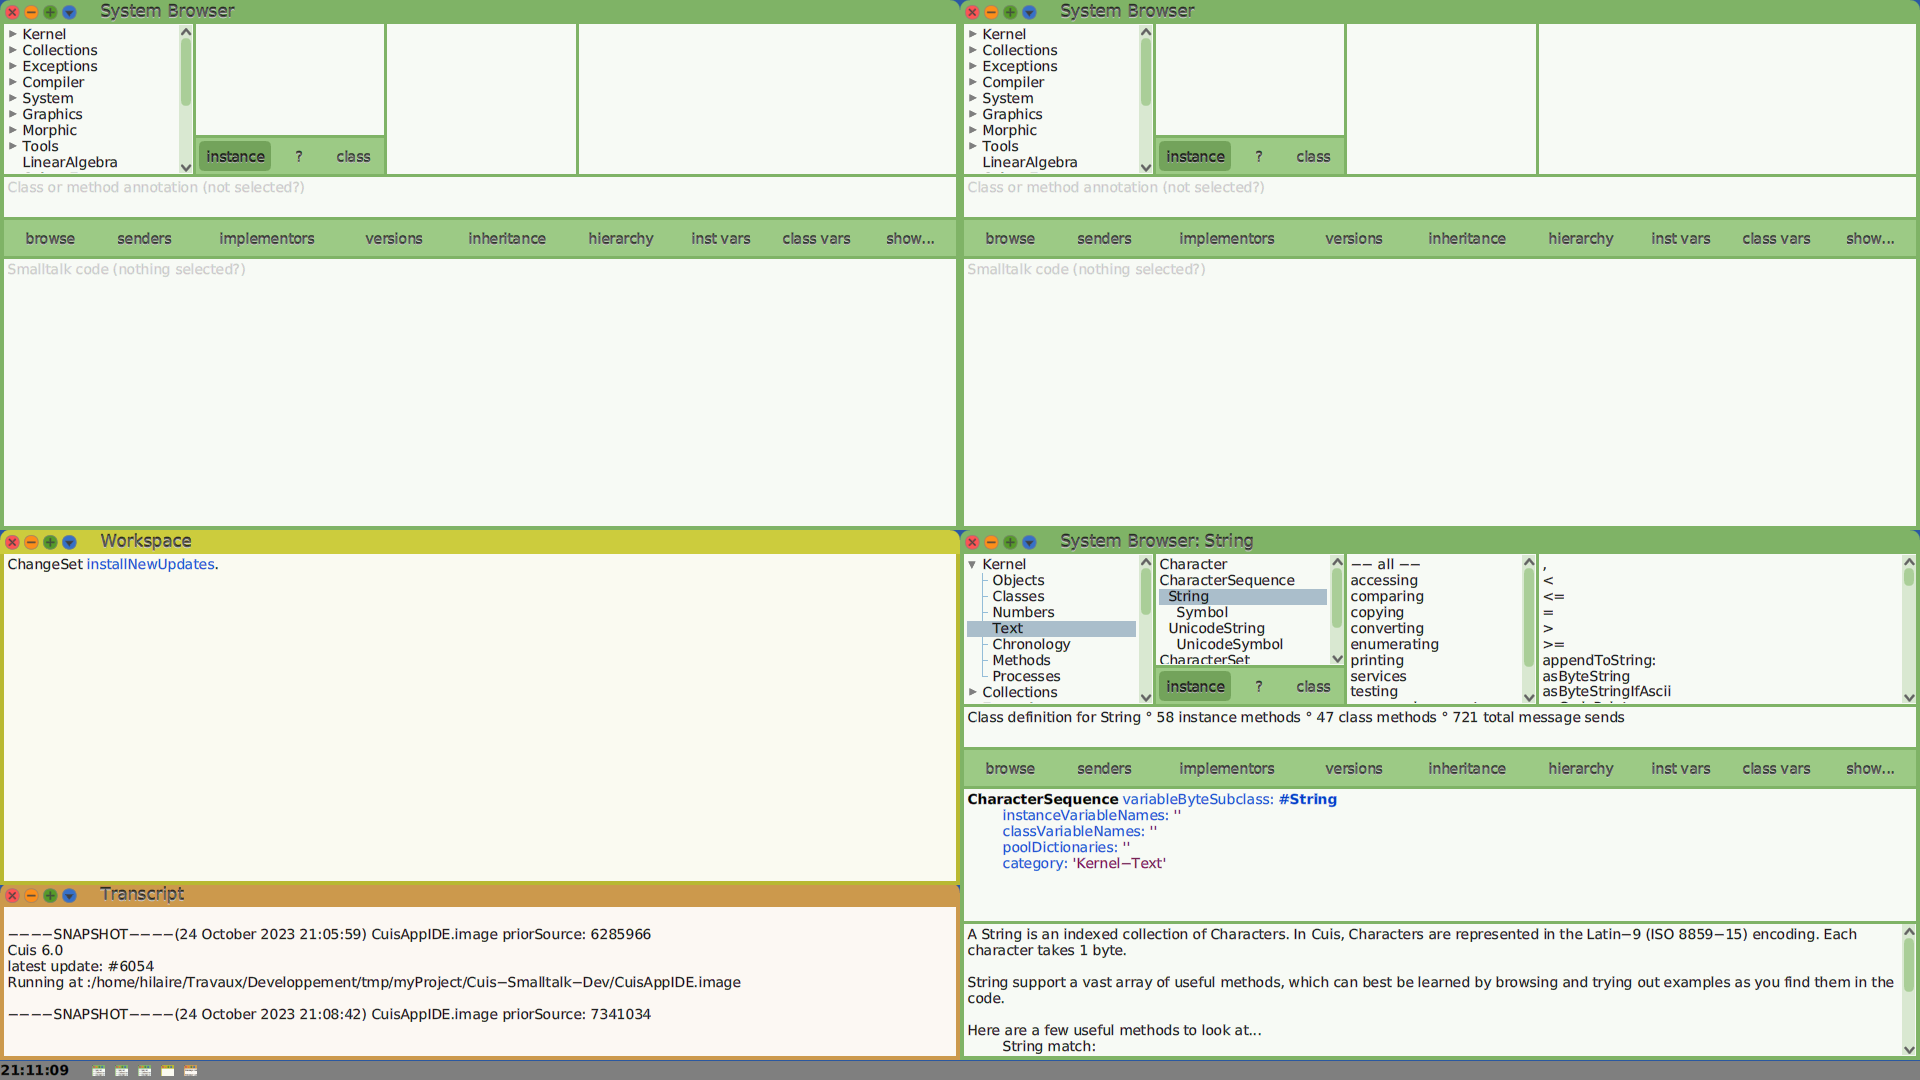
\includegraphics[width=\textwidth]{CuisAppIDE.png}
  \end{center}
\end{frame}
\section{App Design}
% What in there?
\subsection{Design Patterns}
\begin{frame}{Which ones?}
  There are best practices, our CuisApp:
  \begin{itemize}
  \item \textbf{MVP.} Model-View-Presenter for GUI application.
  \item \textbf{Strategy.} Present a set of methods with differents
    implementation depending on the platform.
  \item \textbf{Command.} To undo/redo operation for construction,
    delete, property, merge, move commands
  \end{itemize}

  \tip\ If you are serious about developing an application, you sould
  read a book about design patterns\cite{designPattern}.

\end{frame}
%
\begin{frame}{In Dr. Geo}
  A few more in Dr. Geo:
  \begin{itemize}
  \item \textbf{Factories.} It manufactures new models, keeps record
    of the manufactured models and check for duplicated models.
  \item \textbf{Tools.} Tool and state objects to process
    multiple-steps user input in the canvas. Tools is instantiated by
    the presenter, once the user selected a given construction menu.
  \item \textbf{Builder.} Model builders. Fed by the user input via
    the selected tool to gradually construct an mathematics item.
  \end{itemize}
\end{frame}
\subsection{Model-View-Presenter}
\begin{frame}{General considerations}
  In MVP\cite{guiArch} there are three objects:

  \begin{itemize}
  \item \textbf{Model (Domain object).} It represents the domain. It
    does not know about the view and presenter.
  \item \textbf{View.} It shows the model and the controls (buttons,
    etc.) to manipulate it. It knows about the presenter.
  \item \textbf{Presenter.} It handles the operationss on the model. It
    knows about the model and the view.
  \end{itemize}

  \tip\ The controls in the views are handled by the presenter. Models
  are unaware of the views and presenter.

  \tip\ The Presenter is the entry point in the application.
\end{frame}

\begin{frame}[fragile]{In CuisApp}
  \fontsize{10pt}{8pt}\selectfont
  Our \textbf{Domain} object is around a fileEntry:
  \begin{lstlisting}[language=Smalltalk]
Object subclass: #AppDomain
   instanceVariableNames: 'fileEntry'
   classVariableNames: ''
   poolDictionaries: ''
   category: 'CuisApp-Model'
 \end{lstlisting}
 Our \textbf{View} is around an ImageMorph instance:
 \begin{lstlisting}[language=Smalltalk]
SystemWindow subclass: #AppView
   instanceVariableNames: 'image presenter'
   classVariableNames: ''
   poolDictionaries: ''
   category: 'CuisApp-View'   
 \end{lstlisting}
 And the \textbf{Presenter}, knows about the domain and view through
 the controlsManager:
 \begin{lstlisting}[language=Smalltalk]
Object subclass: #App
   instanceVariableNames: 'domain controlManager cmdManager'
   classVariableNames: ''
   poolDictionaries: ''
   category: 'CuisApp-Presenter'   
 \end{lstlisting}
\end{frame}

\begin{frame}[fragile]{Presenter is central}
    \fontsize{10pt}{8pt}\selectfont
Instantiating the Presenter start the application:
\begin{lstlisting}[language=Smalltalk]
App>>initialize
   domain := AppDomain new.
   controlManager := AppControlManager for: self.
   controlManager installAppView.
   cmdManager := AppCommandManager new presenter: self.
   self view openInWorld 
 \end{lstlisting}
 We use an auxiliary object \texttt{AppControlManager} to arrange the
 view: we keep low the complexity in our \texttt{AppView} and to
 implement alternate arrangement by subclassing
 \texttt{AppControlManager}.
\end{frame}

\begin{frame}[fragile]{Controls}
  \fontsize{10pt}{8pt}\selectfont
  The controls are installed in the view by the
  \texttt{AppControlManager}:
  \begin{lstlisting}[language=Smalltalk]
AppControlManager>>installAppView
| scroller |
   view := AppView for: presenter.
   scroller := PluggableScrollPane new :: 
      layoutSpec: LayoutSpec useAll;
      scroller: view imageMorph.	
   view addMorph: self appToolbar layoutSpec: (LayoutSpec
      fixedHeight: AppSystem iconToolbarSize + 4).
   view addMorph: scroller    
  \end{lstlisting} 
\end{frame}

\begin{frame}[fragile]{The toolbar}
  \fontsize{10pt}{8pt}\selectfont
\begin{lstlisting}[language=Smalltalk]
AppControlManager>>appToolbar
| toolbar |
   toolbar := LayoutMorph newRow 
      separation: 5; 
      yourself.
   self appTools do: [:aTool | 
      aTool == #spacer 
         ifTrue: [toolbar addMorphUseAll: self class spacer]
         ifFalse: [toolbar addMorph: (self button: aTool )]].
^ toolbar    
  \end{lstlisting}

Each tool is described in its own method:
\fontsize{9pt}{8pt}\selectfont
\begin{lstlisting}[language=Smalltalk]
AppControlManager>>openButtonData
" label - iconName - callback - description "
^ {'Open' translated . #open . #openImage .
  'Select a picture to visualize and to operate with.' translated }
\end{lstlisting}

Observe the \texttt{\#translated} message sent to the tool label and
description.
\end{frame}
\begin{frame}[fragile]{The tool}
Observe, the model of the button is the Presenter, action is sent to it:
 \fontsize{9pt}{8pt}\selectfont
  \begin{lstlisting}[language=Smalltalk]
AppControlManager>>button: symbol
"array first = menu label or button label
array second = button form = section mode
array third = symbol callback
array fourth = help string"	
| array |
   array := self perform: (symbol, #ButtonData) asSymbol.
   ^ ButtonMorph 
   model: presenter
      action: array third ::
      enableSelector: (
         symbol == #open ifTrue: [true] ifFalse: [#isButtonActive]);
      icon: (icons get: array second size: AppSystem iconToolbarSize);
      setBalloonText: array fourth;
      ../..
  \end{lstlisting}  
\end{frame}

\begin{frame}[fragile]{Callback}
  Let's take a look to the \texttt{\#openImage} callback:
 \fontsize{9pt}{8pt}\selectfont
  \begin{lstlisting}[language=Smalltalk]
App>openImage
| answer |
   answer := (StandardFileMenu new
      oldFileFrom: AppSystem picturesPath
      withPattern: '*.png *.jpg *.jpeg'
      excludePattern: '.*')
         startUpWithCaption: 'Pick up a picture' translated.
  answer ifNotNil: [
     domain fileEntry: answer directory // answer name.
     cmdManager release]
 \end{lstlisting}
 \fontsize{11pt}{8pt}\selectfont

 \tip\ The domain is updated with the fileEntry of the newly selected
 picture.
 
 Do you think there is a missing piece?
\end{frame}

\begin{frame}[fragile]{Observer pattern}
  How the View knows about a newly selected image? We use the Observer
  pattern. The Domain triggers a \#newImageSelected event:

  \fontsize{10pt}{8pt}\selectfont
  \begin{lstlisting}[language=Smalltalk]
AppDomain>>fileEntry: aFileEntry
   fileEntry := aFileEntry.
   self triggerEvent: #newImageSelected
 \end{lstlisting}
 
 \tip\ Our View is listening to the \texttt{\#newImageSelected} event:
 \begin{lstlisting}[language=Smalltalk]
AppView>>initialize
../..
   self domain when: #newImageSelected
     send: #loadImage to: self
 \end{lstlisting}

  \tip\ And the method \texttt{loadImage} is called:
  \begin{lstlisting}[language=Smalltalk]
AppView>>loadImage
   image image: (ImageReadWriter
      formFromFileEntry: self domain fileEntry).
   self update: #relabel
  \end{lstlisting}
\end{frame}
%
\begin{frame}{Caution with Observer pattern}
  A costly mechanism to use with parsimony, for high level UI
  controls.

  \vspace*{10pt}

  In Dr. Geo canvas, math model (circle below) and its view (morph)
  are not coupled with the observer pattern. Canvas is updated with a
  top-down redraw of the views, it is faster.

  \begin{center}
    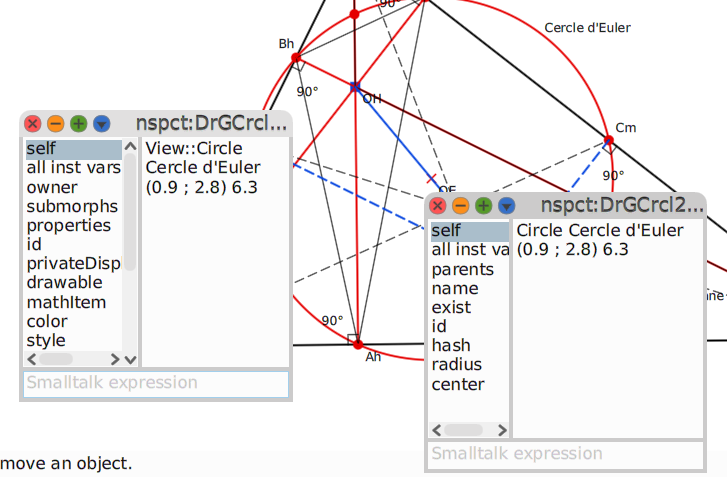
\includegraphics[width=0.6\textwidth]{DrGeoViewModel.png}
  \end{center}
  
\end{frame}
\subsection{Command}
\begin{frame}{General considerations}
  Three objects:
  \begin{itemize}
  \item A command manager, \texttt{AppCommandManager}, to execute
    specific command
  \item A command stack, \texttt{AppCommandStack}, where are stacked the command instances
  \item A hierarchy of command, \texttt{AppCommand}, each specialized
    in one type of operation
  \end{itemize}

  Two important command methods: \texttt{execute} and
  \texttt{unexecute}

  Let's observe it with the rotate right operation.
\end{frame}

\begin{frame}[fragile]{Rotate right callback}
  When the button is pressed in the toolbar, the Presenter's method is
  executed:
\fontsize{10pt}{8pt}\selectfont

 \begin{lstlisting}[language=Smalltalk]
App>>rotateRight
   cmdManager rotateRight 
 \end{lstlisting}
 The command manager create the command, add it to the stack then
 execute it:
 \begin{lstlisting}[language=Smalltalk]
AppCommandManager>>rotateRight
|command|
   command := stack nextPut:
      (AppRotateCommand presenter: presenter).
   command degrees: 90.
   ^ command execute
 \end{lstlisting}
\end{frame}
%
\begin{frame}[fragile]{Rotate right command}
  Observe the execute method. As the execute command is not
  destructive, the unexecute method just rotate the image in the other
  direction:

  \fontsize{10pt}{8pt}\selectfont

 \begin{lstlisting}[language=Smalltalk]
AppRotateCommand>>execute
   self imageMorph image: (self rotatedBy: degrees)

AppRotateCommand>>unexecute
   self imageMorph image: (self rotatedBy: degrees negated)   
 \end{lstlisting}
 
  \fontsize{11pt}{8pt}\selectfont
\tip\  For destructive command as zoom out -- we definitely lose image
 pixels -- we have to keep a copy of the original image:
  \fontsize{10pt}{8pt}\selectfont
  \begin{lstlisting}[language=Smalltalk]
AppZoomOutCommand>>execute
   cacheForm := self imageMorph form.
   self imageMorph image: (cacheForm magnifyBy: 0.5)

AppZoomOutCommand>>unexecute
   self imageMorph image: cacheForm   
\end{lstlisting}

\end{frame}


\section{Localise}
\begin{frame}[fragile]{ Modus operandi 1/2}
\fontsize{10pt}{8pt}\selectfont
  Your application in native language. It need the ``Gettext'' and
  ``System-Locales'' Cuis packages.
  \begin{itemize}
  \item In the code, you write strings in English. 
  \item You send the message \texttt{\#translated} to each string you
    want to be translated:
    \begin{lstlisting}[language=Smalltalk]
... startUpWithCaption: 'Pick up a picture' translated.
    \end{lstlisting}
  \item You define your translation domain based on Class category:
    \begin{lstlisting}[language=Smalltalk]
TextDomainManager
   registerCategoryPrefix: 'CuisApp'
   domain: 'cuisapp'.
 \end{lstlisting}
 \tip\ Our domain is called ``cuisapp''. In the classes of the
 category ``CuisApp'', it tracks the strings with the
 \texttt{\#translated} message sent.
 
\end{itemize}
\end{frame}
%
\begin{frame}[fragile]{ Modus operandi 2/2}
  \begin{itemize}
  \item You export the messages to translate to a .pot template file:
    \begin{lstlisting}[language=Smalltalk]
GetTextExporter exportTemplate
\end{lstlisting}
\tip\ It creates a file \texttt{Cuis-Smalltalk-Dev/po/cuisapp/cuisapp.pot}
\item You copy this file to \texttt{CuisApp/i18n/locale/}
\item To translate to Spanish, you copy this file as ``es.po'' and
  translate it to your native language
\item Add Spanish code ``es'' in the scripts \texttt{buildLocales.sh}
  and \texttt{update-po.sh}
  
  \tip\ Execute \texttt{buildLocales.sh} each time you edited a .po
  file

  \tip\ Execute \texttt{update-po.sh} when the original exported file
  \texttt{cuisapp.pot} was renewed because of additional messages to
  translate or messages edited in the code.
  \end{itemize}
\end{frame}

\begin{lstlisting}[language=Smalltalk]
\end{lstlisting}

\section{Build the application}
\begin{frame}[fragile]{makeBundle}
  The bash script \texttt{makeBundle.sh}:
  \begin{itemize}
  \item Must be executed from \texttt{Cuis-Smalltalk-Dev} directory
  \item Prepare the image:
\begin{verbatim}
./CuisApp/build/makeBundle.sh --build
\end{verbatim}
  \item Make a bundle for GNU/Linux and Windows:
\begin{verbatim}
./CuisApp/build/makeBundle.sh --package gnulinux
./CuisApp/build/makeBundle.sh --package windows
\end{verbatim}
  \end{itemize}
\end{frame}  

\section*{End}
\begin{frame}
  \begin{center}
    \fontsize{16pt}{8pt}\selectfont

  Questions?
\end{center}
\end{frame}
\section{References}
\begin{frame}
  \fontsize{10pt}{8pt}\selectfont
  \begin{thebibliography}{99}

  \bibitem{cuisAppRepo}
    \href{https://github.com/hilaire/CuisApp}{CuisApp template}

  \bibitem{drgeoRepo} \href{https://launchpad.net/drgeo}{\drgeo\
      repository at launchpad with translation management}

  \bibitem{guiArch}
    \href{GUI Architectures}{https://www.martinfowler.com/eaaDev/uiArchs.html}
    
  \bibitem{designPattern}
    Sherman R. Alpert, Kyle Brown, Bobby Woolf,
    \href{https://dl.acm.org/doi/book/10.5555/275616}{The Design
      Patterns Smalltalk Companion}, Addison-Wesley, 1998
    
  \bibitem{cuisRepo}
    \href{https://github.com/Cuis-Smalltalk/Cuis-Smalltalk-Dev/blob/master/Documentation/GettingStarted.md}{Setting
      up and starting Cuis Smalltalk}

  \end{thebibliography}

  
\end{frame}
\end{document}